\documentclass{article}
\usepackage{amsmath}
\usepackage{amssymb}
\usepackage{mathtools}
\usepackage{amsfonts}
\usepackage{stmaryrd}
\usepackage[french]{babel}
\usepackage{cancel}
\usepackage{stackrel}
\usepackage{graphicx}
\graphicspath{ {./screens/} }

\makeatletter

%%%%%%%%%%%%%%%%%%%%%%%%%%%%%% LyX specific LaTeX commands.
%% Because html converters don't know tabularnewline
\providecommand{\tabularnewline}{\\}

\makeatother

\begin{document}


%\title {PROJET GM3 / S2V2 \\[1ex] \large MSRO - Simulation et estimation dans le cadre de la loi de Pareto}
%\author{Tom BOUMBA et Angelo CASTINO}
%\date{\today}
%\maketitle


\begin{titlepage}
	\centering
	\vfill
	{
		\bfseries\Large
		Simulation et Estimation \\
		Loi de Pareto \\
	}    
	\vskip1cm
	{	
		\bfseries\large
		Tom Boumba et Angelo Castino \\
	}
	\vskip2cm
		Encadré par : Pr. Bruno Portier, Mr. Michel Bobia \\
		PROJET GM3 / S2V2 - MSRO\\
	\vfill
	
\includegraphics[width=4cm]{logo_insa}
	\vfill
	\vfill
\end{titlepage}


\pagebreak

\tableofcontents

\pagebreak

\section{Introduction}

A la fin du $XIX^{e}$ siècle, l'économiste italien Vilferdo Pareto a mis au point un principe qui porte aujourd'hui son nom : Le principe de Pareto.
En effet, en analysant les données fiscales des plus puissants pays européens, il a remarqué que nonobstant une certaine variabilité selon le pays, le pourcentage de la population possédant une richesse superieure ou égale à un $x$ donné était proportionnel à $\frac{A}{x^{\alpha}}$ ($A$ étant une constante, et le coefficient $\alpha$ variant selon les pays).
Ses travaux ont inspiré beaucoup de ses collègues qui ont mené des recherches approfondies sur ce phénomène, ce qui a mené à la formalisation de la loi de Pareto, aujourd'hui très importante en économie, et permettant par exemple d'optimiser la gestion de stocks, de clients ou de temps.
Une loi de Pareto est donc aujourd'hui formalisée par la théorie des probabilités comme étant une loi à densité hyperbolique permettant de modéliser probabilistiquement une relation de cause à effet asymétrique.
Dans ce projet, nous étudions tout d'abord les caractéristiques théoriques d'une variable aléatoire suivant une loi de Pareto (espérance, variance, fonction de répartition inverse, estimateur de maximum de vraissemblance). On trouve notamment que le paramètre $\alpha$ de la loi doit être strictement supérieur à $2$ pour que la variable admette une espérance et une variance finies, et que l'estimateur de maximum de vraissemblance du paramètre $\beta=\frac{1}{\alpha}$ est sans biais et convergent.
Ensuite, nous nous intéressons à la simulation d'une telle variable aléatoire par la méthode de l'inversion, qui est applicable car la fonction de répartition de la variable est continue et strictement croissante.
Enfin, en nous basant sur un échantillon de causes observées, qui sont supposément des réalisations indépendantes d'une variable aléatoire suivant une loi de Pareto, on cherche à déterminer le paramètre $\alpha$ de la loi en question par la méthode de l'estimation par maximum de vraissemblance. Cela nous permet de mettre de évidence le caractère sans biais et convergent de l'estimateur de maximum de vraissemblance. 

\pagebreak

\section{Partie théorique : étude mathématique}

\subsection{Étude probabiliste}

1. Soient $\alpha$ et $\theta$ deux réels strictements positifs.
Déterminer le réel $C$ pour que la fonction : $x\rightarrow\begin{cases}
\frac{C}{x^{\alpha+1}} & si\ x\geq\theta\\
0 & sinon.
\end{cases}$ soit une densité de probabilité.

On sait que $f$ est une densité si :
\begin{align*}
\int_{-\infty}^{+\infty}f(t)dt & =1\Leftrightarrow\int_{\theta}^{+\infty}\frac{C}{x^{\alpha+1}}dx=1\\
\Leftrightarrow & C\int_{\theta}^{+\infty}\frac{1}{x^{\alpha+1}}dx=1\\
\Leftrightarrow & C[\frac{-1}{\alpha x^{\alpha}}]_{\theta}^{+\infty}=1\\
\Leftrightarrow & \frac{C}{\alpha\theta^{\alpha}}=1\\
\Leftrightarrow & C=\alpha\theta^{\alpha}
\end{align*}
On obtient que :$f(x)=\begin{cases}
\frac{\alpha}{\theta}(\frac{\theta}{x})^{\alpha+1} & si\ x\geq\theta\\
0 & sinon
\end{cases}$\\
Dans toute la suite, on notera cette densité $f$.\\
\\
\textbf{Définition} : On dit que la variable aléatoire X suit une
loi de Pareto de paramètres $\alpha$ et $\theta$ si et seulement
si sa densité est $f.$ On notera alors $X\sim P(\alpha,\theta).$\\
\\
Dans ce qui suit, X désignera une variable aléatoire de loi $P(\alpha,\theta)$\\
\\
2. Dans quelle contexte cette loi est-elle utilisée? Donner des exemples
de modélisation avec une telle loi.\\

Après quelques recherches, on apprend que cette loi est utilisé en
économie principalement. Elle est néanmoins très discutée car beaucoup
la trouvent trop imprécise. A l'aide de la loi de Pareto on peut notemment
modeliser de la gestion de stock, de ventes, de projet ou de production.
On appelle aussi cette loi la loi des 80-20 car elle permet d'observer
que 80\% des effets sont le produit de seulement 20\% des causes.
En effet, si on modélise un problème comme étant causé par les valeurs
que peuvent prendre X, on voit qu'après $\theta$, approximativement
20\% des valeurs de cause constituent 80\% de l'intégrale de la densité
de probabilité du problème (voir figure \ref{fig:schema-densite}).
On peut généraliser ce raisonnement pour différentes valeurs de $\alpha$
(on a alors des proportions différentes de 80-20).
\clearpage
\begin{figure}
\caption{Densité de loi de Pareto schématisée\label{fig:schema-densite}}

\centering{}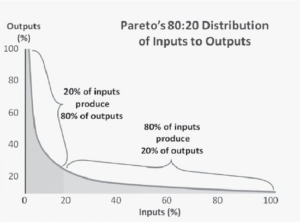
\includegraphics{schema_loi}
\end{figure}
3. A quelle condition la variable X posède-t-elle une espérance ?
une variance ? On se placera sous cette dernière condition dans la
suite.
\begin{itemize}
\item X admet une espérance si :
\begin{align*}
 & \int_{-\infty}^{+\infty}|x|f(x)dx\ converge\\
\Leftrightarrow & \int_{\theta}^{+\infty}|x|\frac{\alpha}{\theta}(\frac{\theta}{x})^{\alpha+1}dx=\theta^{\alpha}\alpha\int_{\theta}^{+\infty}\frac{1}{x^{\alpha}}dx\ \ \ \ ,(\theta>0\Leftrightarrow|x|=x)\ converge\\
\Leftrightarrow\  & \alpha>1\ (Int\acute{e}grale\ de\ Riemann)
\end{align*}
\\
X admet une espérance si $\alpha>1$ et cette espérance vaut :\\
\[
E(X)=\int_{-\infty}^{+\infty}xf(x)dx
\]
\item X admet une variance si X admet une espérance et si :
\begin{align*}
 & \int_{-\infty}^{+\infty}(x-E(X))^{2}f(x)dx\ converge\\
\Leftrightarrow & \int_{\theta}^{+\infty}x^{2}f(x)dx+E(X)^{2}\int_{\theta}^{+\infty}f(x)dx-2E(X)\underset{E(X)}{\underbrace{\int_{\theta}^{+\infty}xf(x)dx}}=\int_{\theta}^{+\infty}x^{2}f(x)dx-E(X)^{2}\ converge\\
\Leftrightarrow & \int_{\theta}^{+\infty}x^{2}f(x)dx\ converge\\
\Leftrightarrow & \theta^{\alpha}\alpha\int_{\theta}^{+\infty}\frac{1}{x^{\alpha-1}}\ converge\\
\Leftrightarrow & \ \alpha-1>1\ (Int\acute{e}grale\ de\ Riemman)\\
\Leftrightarrow & \,\alpha>2
\end{align*}
\\
X admet une variance si $\alpha>2$ et cette variance vaut :
\[
V(X)=\int_{-\infty}^{+\infty}(x-E(x))^{2}f(x)dx=E(X^{2})-E(X)^{2}
\]
\end{itemize}
4. Calculer l'espérance et la variance de X.
\begin{itemize}
\item Calcul de l'espérance :
\begin{align*}
E(X) & =\theta^{\alpha}\alpha\int_{\theta}^{+\infty}\frac{1}{x^{\alpha}}dx\\
= & \theta^{\alpha}\alpha[\frac{-1}{(\alpha-1)x^{\alpha-1}}]_{\theta}^{+\infty}\\
= & \theta^{\alpha}\alpha\frac{1}{(\alpha-1)\theta^{\alpha-1}}\\
= & \frac{\theta\alpha}{(\alpha-1)}
\end{align*}
\item Calcul de la variance :
\begin{align*}
V(x)= & E(X^{2})-E(X)^{2}\\
E(X^{2})= & \frac{\theta^{2}\alpha}{(\alpha-2)}\\
V(X)= & \frac{\theta^{2}\alpha}{(\alpha-2)}-\frac{\theta^{2}\alpha^{2}}{(\alpha-1)^{2}}\\
V(X)= & \frac{\theta^{2}\alpha(\alpha-1)^{2}-\theta^{2}\alpha^{2}(\alpha-2)}{(\alpha-1)^{2}(\alpha-2)}\\
V(X)= & \frac{\alpha\theta^{2}}{(\alpha-1)^{2}(\alpha-2)}
\end{align*}
\end{itemize}
5. Calculer la fonction de répartition F de X.

La fonction de répartition, notée $F_{X}(x)$ se calcule suivant la
formule suivante :

\begin{align*}
F_{X}(x)= & P(X\leq x)=\int_{-\infty}^{x}f(t)dt\\
= & \begin{cases}
0 & si\ x<\theta\\
\int_{\theta}^{x}\frac{\alpha}{\theta}(\frac{\theta}{t})^{\alpha+1}dt & si\ x\geq\theta
\end{cases}\\
= & \begin{cases}
0 & si\ x<\theta\\
\alpha\theta^{\alpha}[\frac{-1}{\alpha t^{\alpha}}]_{\theta}^{x}=\frac{\bcancel{\alpha\theta^{\alpha}}}{\bcancel{\alpha\theta^{\alpha}}}-\frac{\bcancel{\alpha}\theta^{\alpha}}{\bcancel{\alpha}x^{\alpha}} & si\ x\geq\theta
\end{cases}\\
= & \begin{cases}
0 & si\ x<\theta\\
1-(\frac{\theta}{x})^{\alpha} & si\ x\geq\theta
\end{cases}
\end{align*}
\\
6. Déterminer la fonction réciproque de F.

\begin{align*}
y= & 1-(\frac{\theta}{x})^{\alpha}\\
(\frac{\theta}{x})^{\alpha}= & 1-y\\
x^{\alpha}= & \frac{\theta^{\alpha}}{1-y}\\
x= & \frac{\theta}{(1-y)^{1/\alpha}}
\end{align*}

On a donc : 
\[
F^{-1}(x)=\frac{\theta}{(1-x)^{1/\alpha}}
\]


\subsection{Simulation d'une valeur d'une variable de loi de Pareto}

L\textquoteright objet de ce paragraphe est de proposer une méthode
de construction d\textquoteright une valeur d\textquoteright une variable
aléatoire de loi P($\alpha$,$\theta$).\\
\\
7. Expliquer de manière formelle comment simuler une valeur d\textquoteright une
variable aléatoire de loi P($\alpha$,$\theta$).

On va appliquer la méthode d'inversion. 

Soit X une variable réelle de loi continue et strictement croissante.
Alors si U est de loi uniforme sur {[}0,1{]}, la variable $F^{-1}(U)$
a la même loi que X.

Dans le cadre de la loi de Pareto :

\[
\begin{cases}
F(\theta^{-})=0\\
F(\theta)=1-(\frac{\theta}{\theta})^{\alpha}=0
\end{cases}
\]

Donc F est continue en $\theta$, de plus F est continue de manière
triviale sur $\mathbb{R}\backslash\{\theta\},$donc F est continue
sur $\mathbb{R}$.

F est également strictement croissante sur $[\theta,+\infty[$ de
manière évidente.

On peut donc appliquer la méthode d'inversion à la loi de Pareto pour
en simuler une valeur $x$ en simulant une réalisation u de U et en
posant $x=F^{-1}(u)=\frac{\theta}{(1-u)^{1/\alpha}}$.

\subsection{Étude statistique}

On considère $n$ données réelles $x_{1},x_{2},...,x_{n}.$ On fait
l'hypothèse que ces données sont les réalisations de $n$ variables
aléatoires $X_{1},X_{2},...,X_{n},$indépendantes et de même loi $P(\alpha,\theta=1).$
On suppose que le paramètre $\alpha$ est inconu et on s'intéresse
au problème de son estimation par la méthode du maximum de vraisemblance.\\
\\
8. Ecrire la log-vraisemblance de l\textquoteright échantillon et
trouver l\textquoteright estimation du maximum de vraisemblance de
$\alpha$. En déduire alors l\textquoteright estimateur du maximum
de vraisemblance du paramètre $\alpha$. On le notera $\widehat{\alpha}_{n}$.\\
\\
\begin{align*}
L(x,\alpha)= & \prod_{j=1}^{n}\alpha(\frac{1}{x_{j}})^{\alpha+1}\\
log(L(x,\alpha))= & nln(\alpha)-\sum_{j=1}^{n}(\alpha+1)ln(x_{j})\\
= & nln(\alpha)-(\alpha+1)s_{n}\ avec\ s_{n}=\sum_{j=1}^{n}ln(x_{j})\\
t_{n}= & arg\ \underset{z\in[1,+\infty]}{max(LL(x,z))}\\
g(z)= & nln(z)-(z+1)s_{n}\\
g^{\prime}(z)= & \frac{n}{z}-s_{n}\\
g^{\prime\prime}(z)= & \frac{-n}{z^{2}}
\end{align*}
Donc $g^{\prime}(z)=0\Leftrightarrow z=\frac{n}{s_{n}}$ et $g^{\prime\prime}(z)<0.$
L'unique valeur $t_{n}$ qui maximise la vraisemblance sachant $x_{1},x_{2},...,x_{n}$
est donc égale à $t_{n}=\frac{n}{s_{n}}$\\
On peut alors construire un estimateur du maximum de vraisemblance
de $\alpha$ noté $\widehat{\alpha}_{n}$: $\widehat{\alpha}_{n}=\frac{n}{\sum_{j=1}^{n}log(X_{j})}$\\
9. Calculer $E[log(X_{1})]$ et $Var(log(X_{1})).$\\
\\
\begin{align*}
E(log(X_{1}))= & \int_{1}^{+\infty}\alpha ln(x)(\frac{1}{x}){}^{\alpha+1}dx\\
= & \alpha\int_{1}^{+\infty}ln(x)(\frac{1}{x})^{\alpha+1}dx\\
\text{On va procéder par intégration par parties :} & u(x)=ln(x),u^{\prime}(x)=\frac{1}{x},v^{\prime}(x)=\frac{1}{x^{\alpha+1}},v(x)=\frac{-1}{\alpha x^{\alpha}}\\
\int_{1}^{+\infty}ln(x)(\frac{1}{x})^{\alpha+1}dx= & [\frac{-ln(x)}{\alpha x^{\alpha}}]_{1}^{+\infty}+\int_{1}^{+\infty}\frac{1}{\alpha x^{\alpha+1}}dx\\
= & 0+[\frac{-1}{\alpha^{2}x^{\alpha}}]_{1}^{+\infty}=\frac{1}{\alpha^{2}}\\
\text{donc \ensuremath{E(log(X_{1}))=}} & \frac{1}{\alpha}
\end{align*}
Calcul de $Var(log(X_{1}))$ :
\begin{align*}
Var(log(X_{1}))= & E((log(X_{1}))^{2})-E(log(X_{1}))^{2}\\
E((log(X_{1}))^{2})= & \alpha\int_{1}^{+\infty}ln^{2}(x)(\frac{1}{x})^{\alpha+1}dx\\
= & \underset{0}{\alpha(\underbrace{[\frac{-ln^{2}(x)}{\alpha x^{\alpha}}]_{1}^{+\infty}}}+\int_{1}^{+\infty}\frac{2ln(x)}{\alpha x^{\alpha+1}}dx)\\
= & \frac{2}{\alpha^{2}}\\
Var(log(X_{1}))= & \frac{1}{\alpha^{2}}
\end{align*}
\\
\\
10. Proposer un estimateur sans biais et convergent du paramètre $\beta=\frac{1}{\alpha}$.
On notera cet estimateur $B_{n}$et $b_{n}$sa réalisation.\\
\\
\[
B_{n}=\frac{1}{n}\sum_{i=1}^{+\infty}log(X_{i})
\]
\\
$B_{n}$ est un estimateur du paramètre $\beta=\frac{1}{\alpha}$
sans biais et convergent. En effet, $E(log(X_{1}))=\frac{1}{\alpha}$
donc par linéarité de l'espérance, on a\\
\\
\[
E(B_{n})=\frac{\bcancel{n}}{\bcancel{n}}\beta=\beta
\]
\\
De même, puisque les variables $X_{i}$ indépendantes, on a la linéarité
de la variance de leur somme, donc\\
\\
\[
Var(B_{n})=\frac{n}{n^{2}}\beta^{2}\rightarrow0
\]
\\
11. Enoncer le TLC que satisfait cet estimateur.\\
\\
$E(log(X_{1})^{2})<\infty$ car la variance de $log(X_{i})$ existe.
Cette variable admet donc un momet d'ordre 2. $B_{n}$vérifie donc
le Théorème limite centrale suivant :\\
\[
\sqrt{n}(\underset{B_{n}}{\underbrace{\frac{1}{n}\sum_{j=1}^{n}log(X_{i})}}-E(log(X_{i})))\stackrel[n\rightarrow\infty]{\mathcal{L}}{\rightarrow}N(0,Var(log(X_{i})))
\]

\[
\sqrt{n}(B_{n}-\beta)\stackrel[n\rightarrow\infty]{\mathcal{L}}{\rightarrow}N(0,\beta^{2})
\]
\\
12. Proposer un estimateur du paramètre $\alpha$. On le notera $A_{n}$.\\
\\
\[
A_{n}=B_{n}^{-1}=\frac{n}{\sum_{i=1}^{n}log(X_{i})}=\widehat{\alpha_{n}}
\]
\\
\\
13. En déduire la convergence de $A_{n}$vers $\alpha$ et énoncer
le TLC que satisfait $A_{n}.$

D'après la loi forte des grands nombres, on a :

\begin{align*}
B_{n} & \stackrel[n\rightarrow\infty]{p.s}{\rightarrow}\beta\\
\text{donc }\frac{1}{B_{n}}=A_{n} & \stackrel[n\rightarrow\infty]{p.s}{\rightarrow}\frac{1}{\beta}=\alpha
\end{align*}

$A_{n}$converge donc bien vers $\alpha$.

On a :

\[
\sqrt{n}(B_{n}-\beta)\stackrel[n\rightarrow\infty]{\mathcal{L}}{\rightarrow}N(0,\beta^{2})
\]

On utilise la delta-méthode en utilisant $g(x)=\frac{1}{x}$, dérivable
en $\alpha$ de manière évidente ($\alpha>0$)

\[
\sqrt{n}(\frac{1}{B_{n}}-\frac{1}{\beta})\stackrel[n\rightarrow\infty]{\mathcal{L}}{\rightarrow}N(0,(-\frac{1}{\beta^{2}})^{2}\beta^{2})
\]

On obtient donc finalement :

\[
\sqrt{n}(A_{n}-\alpha)\stackrel[n\rightarrow\infty]{\mathcal{L}}{\rightarrow}N(0,\alpha^{2})
\]


\subsection{Récapitulatif de la partie mathématique}

\begin{tabular}{|c|c|c|}
\hline 
Fonction de densité & $f(x)$ & $\begin{cases}
\frac{\alpha}{\theta}(\frac{\theta}{x})^{\alpha+1} & si\ x\geq\theta\\
0 & sinon
\end{cases}$\tabularnewline
\hline 
Fonction de répartition & $F(x)$ & $\begin{cases}
0 & si\ x<\theta\\
1-(\frac{\theta}{x})^{\alpha} & si\ x\geq\theta
\end{cases}$\tabularnewline
\hline 
Fonction inverse de la fonction de répartition & $F^{-1}(x)$ & 

$F^{-1}(x)=\frac{\theta}{(1-x)^{1/\alpha}}$

\tabularnewline
\hline 
Esperance & $E(X)$ & $\frac{\theta\alpha}{(\alpha-1)}$ $(\alpha>1)$\tabularnewline
\hline 
Variance & $V(x)$ & $\frac{\alpha\theta^{2}}{(\alpha-1)^{2}(\alpha-2)}$$(\alpha>2)$\tabularnewline
\hline 
Estimateur du paramètre $\alpha$ & $A_{n}$ & $\frac{n}{\sum_{i=1}^{n}log(X_{i})}$\tabularnewline
\hline 
\end{tabular}

\pagebreak

\section{Résultats numériques}

Nous avons implémenté la méthode d'inversion pour la simulation et l'estimation par maximum de vraissemblance sous R.

\subsection{Simulation de la loi de Pareto}

Nous avons simulé un échantillon de $400$ réalisations de la loi de Pareto $\mathcal{P}(\alpha,\theta=1)$ par la méthode de l'inversion, puis affiché les fréquences des valeurs obtenues sous la forme d'un histogramme de $20$ classes. Nous avons ensuite superposé la courbe représentative de la densité de la loi $\mathcal{P}(\alpha,\theta=1)$ sur le graphique.

Voici l'un des graphiques que nous avons obtenus (figures $2$ et $3$, pour $\alpha=2$).

\clearpage

\begin{figure}[!h]
\begin{center}
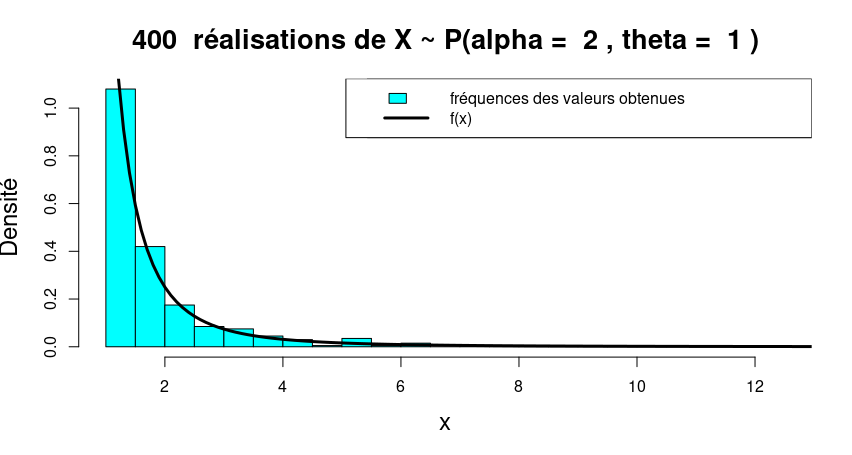
\includegraphics[width=12cm]{plot_hist}
\caption{Affichage de l'histogramme et de la courbe de densité de $\mathcal{P}(\alpha,\theta=1)$}
\vspace{\floatsep}
\vspace{\floatsep}
\vspace{\floatsep}
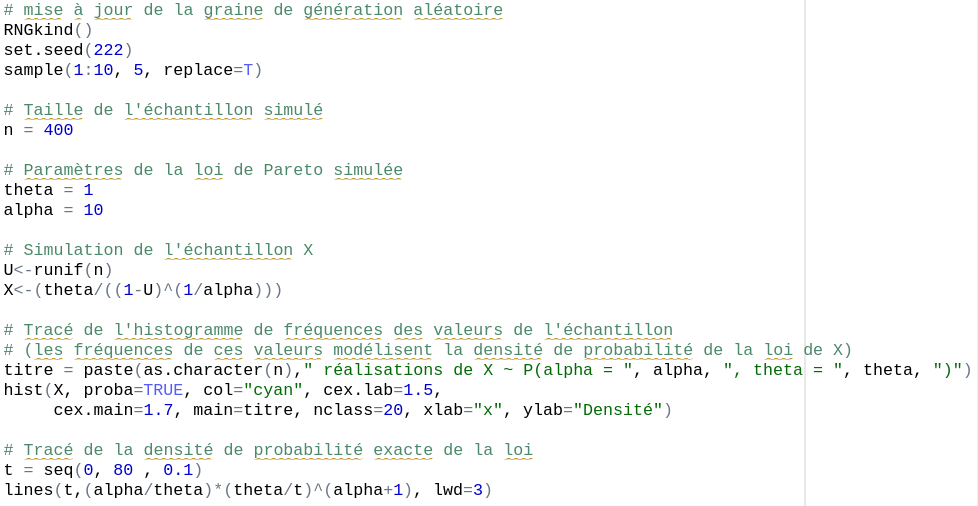
\includegraphics[width=12cm]{code_hist}
\caption{Code R permettant de générer les simulations de $\mathcal{P}(\alpha,\theta=1)$}
\end{center}
\end{figure}

Les résultats graphiques confirment que la simulation par la méthode de l'inversion fonctionne correctement car l'histogramme suit la courbe de la densité de $\mathcal{P}(\alpha,\theta=1)$. De plus, la valeur de $\alpha$ choisie a une influence sur la magnitude des valeurs obtenues, mais pas sur leur répartition (voir annexe figures $9$ et $10$). On remarque toutefois que puisque les valeurs simulées le sont de manière aléatoire (car la variable $X$ est aléatoire), on obtient un histogramme différent si on change la graine de génération aléatoire, ce qui illustre le phénomène de la fluctuation d'échantillonnage (voir annexe figure $8$).

\subsection{Estimation du paramètre $\alpha$}

\subsubsection{Graphique d'évolution de l'estimateur}

Tout d'abord, nous avons simulé un échantillon de $400$ réalisations de $X \sim \mathcal{P}(\alpha,\theta=1)$. Ensuite, nous avons utilisé cet échantillon pour calculer les valeurs de l'estimation de $\alpha$ par maximum de vraissemblance $A_n$ pour $n$ allant de $1$ à $40$, puis pour $n$ allant de $1$ à $400$.

Nous avons obtenu ces graphiques pour l'une des exécutions (figures $4$ et $5$, pour $\alpha=2$). 

\clearpage

\begin{figure}[!h]
\begin{center}
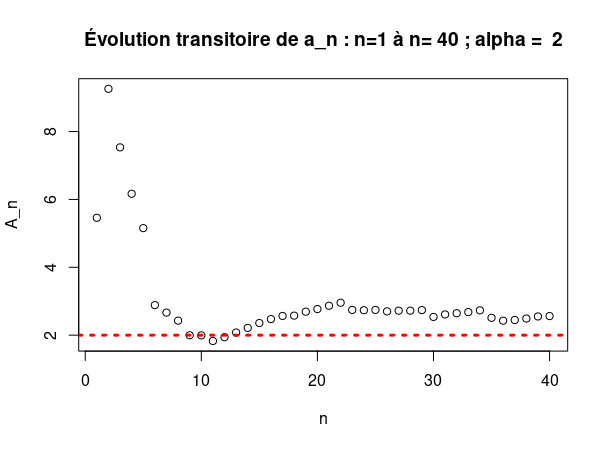
\includegraphics[width=6cm]{plot_graphique_transi}
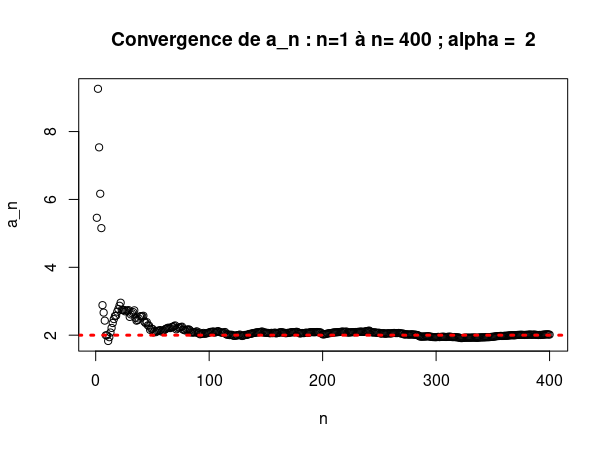
\includegraphics[width=6cm]{plot_graphique_conv}
\caption{Affichage des courbes d'évolution de $a_n$}
\vspace{\floatsep}
\vspace{\floatsep}
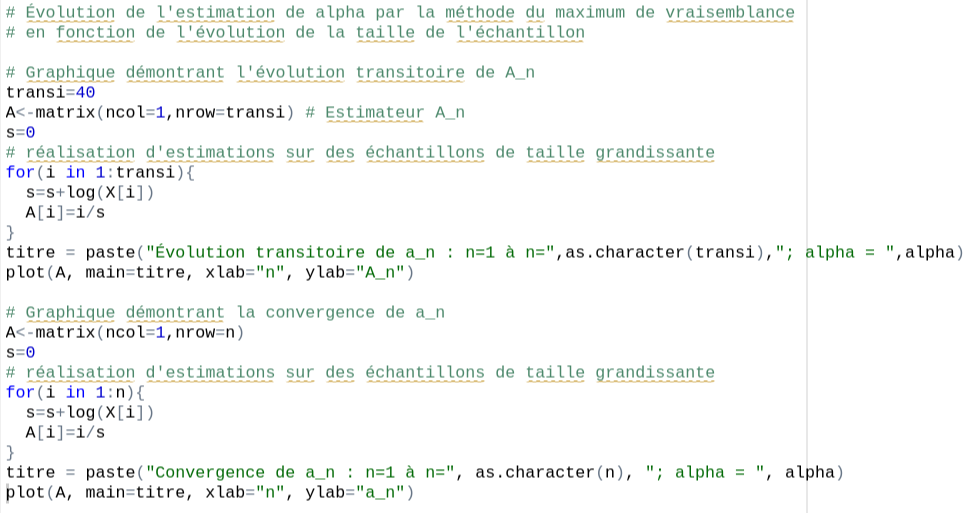
\includegraphics[width=12cm]{code_graphique}
\caption{Code R permettant de générer les valeurs de $a_n$}
\end{center}
\end{figure}

On peut voir que l'estimateur est bien convergent car au fur et à mesure que $n$ augmente, $a_n$ se rapproche asymptotiquement de $\alpha$ (ici $2$). Toutefois, pour des petites valeurs de $n$, on peut voir un manque de performance de l'estimateur, ce qui illustre son caractère transitoire : il faut que $n$ dépasse un certain "seuil" (qui est empirique, on pourrait dire $n=50$) pour que l'estimateur devienne performant. Ici encore, selon les exécutions, en changeant la graine de génération aléatoire, on obtient des résultats différents (la fluctuation d'échantillonnage) mais tous nous permettent d'obtenir cette même conclusion (voir annexe figure $11$), et la valeur d'$\alpha$ n'importe pas (voir annexe figures $11$ et $12$).

\subsubsection{Boîtes à moustaches}

Tout d'abord, nous avons simulé $400$ échantillons de $1000$ simulations de $X \sim \mathcal{P}(\alpha,\theta=1)$. Nous avons ensuite calculé les valeurs de $a_n$ pour $n$ allant de $1$ à $1000$ pour chacun des $400$ échantillons (nous avons appelé "échantillon d'estimations de $\alpha$" l'ensemble des $400$ valeurs $a_n$ générées pour un $n$ donné). Enfin, nous avons représenté les échantillons d'estimations par des boîtes à moustaches pour $n$ prenant certaines valeurs arbitraires ($25$, $50$, $100$, $200$, $500$, et $1000$).

Voici les boîtes à moustaches que nous avons obtenues pour l'une des exécutions (voir figures $6$ et $7$, pour $\alpha=2$).

\clearpage

\begin{figure}[!h]
\begin{center}
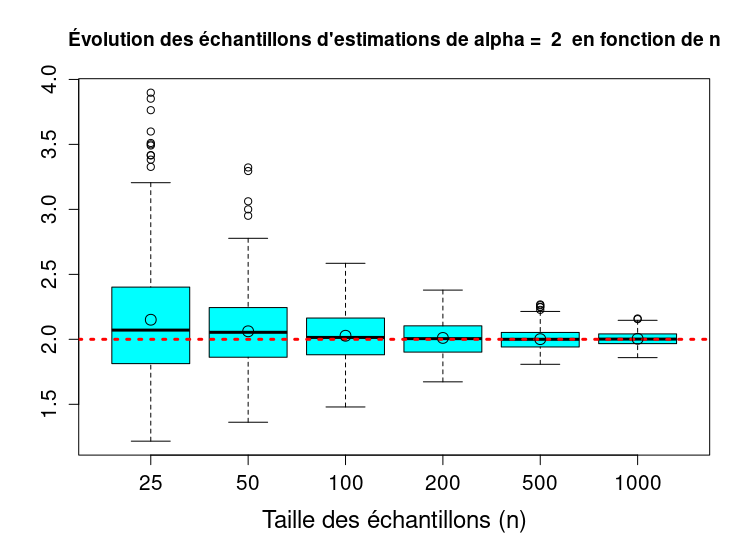
\includegraphics[width=12cm]{plot_box}
\caption{Représentation des échantillons d'estimations de $\alpha$ par des boîtes à moustaches}
\vspace{\floatsep}
\vspace{\floatsep}
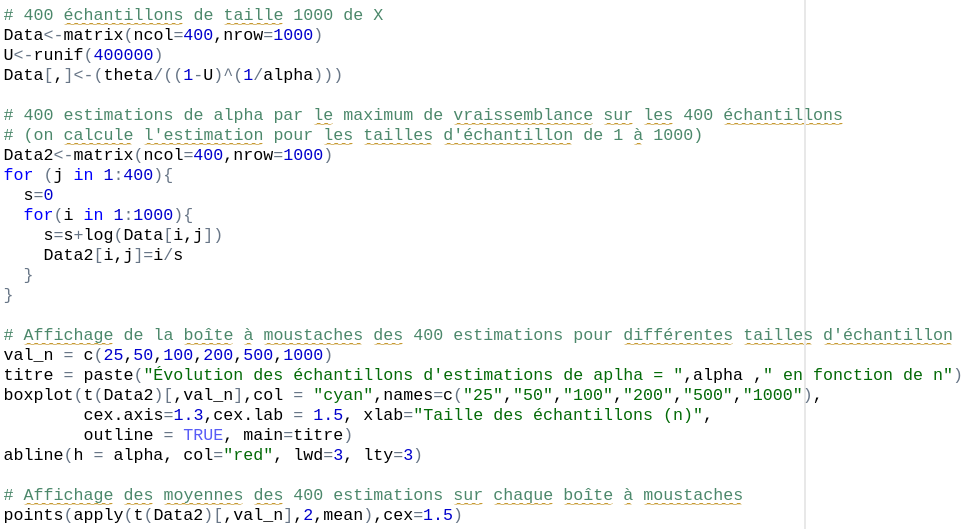
\includegraphics[width=12cm]{code_box}
\caption{Code R permettant de générer les valeurs de $a_n$}
\end{center}
\end{figure}

On observe le caractère sans biais de l'estimateur $a_n$, car même pour des valeurs de $n$ "petites", la moyenne des $400$ estimations calculées est proche de $\alpha$. De plus, on observe la convergence de l'estimateur car lorsque $n$ augmente, la taille des boîtes à moustaches diminue, ce qui illustre une baisse de l'influence des fluctuations d'échantillonnage sur les résultats obtenus lorsque $n$ augmente, ce qui nous confirme que la variance de l'estimateur tend vers $0$ lorsque $n$ augmente. Les résultats obtenus lors d'exécutions différentes (à cause des fluctuations d'échantillonnage, voir annexe figure $13$) nous permettent de tirer des conclusions simillaires, et la valeur de $\alpha$ n'a pas d'influence sur nos conclusions (voir annexe figure $14$).

\pagebreak

\section{Conclusion}

Après avoir étudié les caractéristiques théoriques d'une variable aléatoire suivant une loi de Pareto, nous avons donc pu simuler une telle variable aléatoire, et estimer son paramètre $\alpha$ par la méthode du maximum de vraissemblance. Nous avons constaté une variation des résultats obtenus selon les exécutions effectuées causée par la fluctuation d'échantillonnage (que ce soit pour la simulation ou pour l'estimation de $\alpha$). Mais malgré ces fluctuations, nous avons constaté par l'expérience d'une part la performance de la méthode de simulation par inversion d'une variable alétoire de loi de Pareto, et d'autre part le caractère sans biais et la convergence de l'estimateur de maximum de vraissemblance du paramètre $\alpha$. 

\section{Bibliographie}

\begin{itemize}
\item[-] Cours magistral, travaux dirigés, et travaux pratiques encadrés de Statistique Inférentielle de GM3, Pr. Bruno PORTIER, 2022
\end{itemize}

\pagebreak

\section{Annexe}

\subsection{Figures}

\begin{figure}[!ht]
\begin{center}
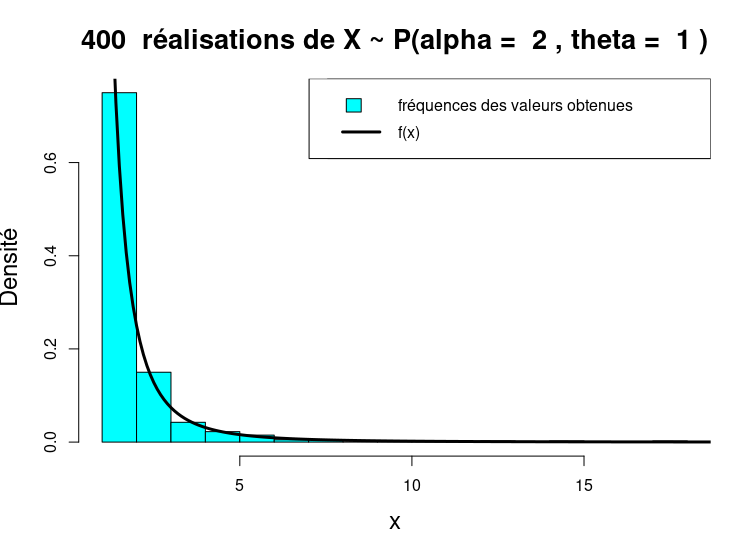
\includegraphics[width=10cm]{plot_hist_1}
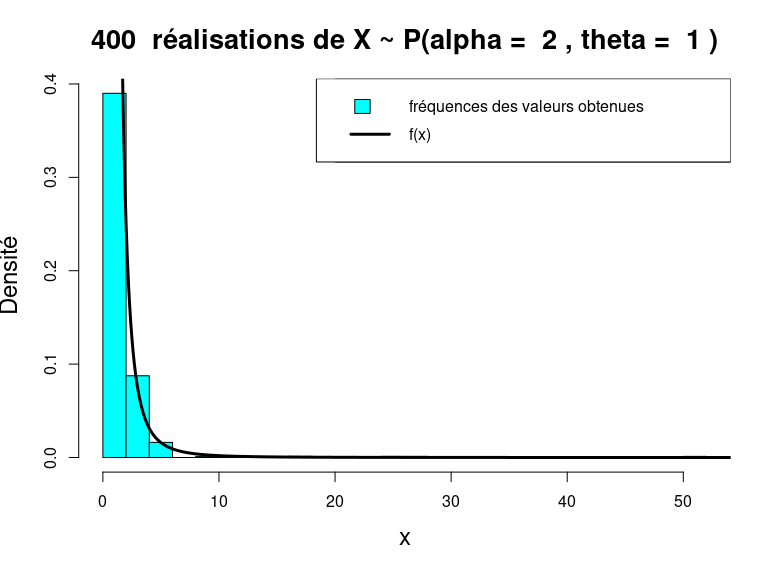
\includegraphics[width=10cm]{plot_hist_2}
\caption{D'autres simulations d'une variable $X \sim \mathcal{P}(\alpha=2,\theta=1)$}
\end{center}
\end{figure}

\clearpage

\begin{figure}[!ht]
\begin{center}
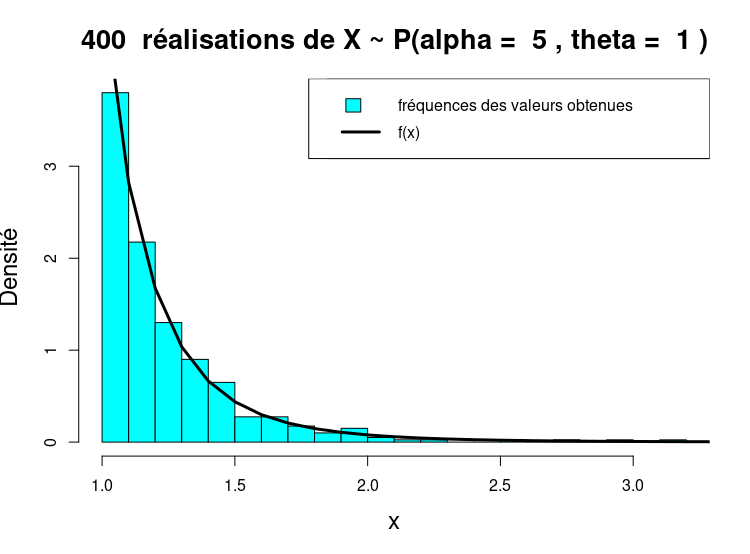
\includegraphics[width=11cm]{plot_hist_1_a5}
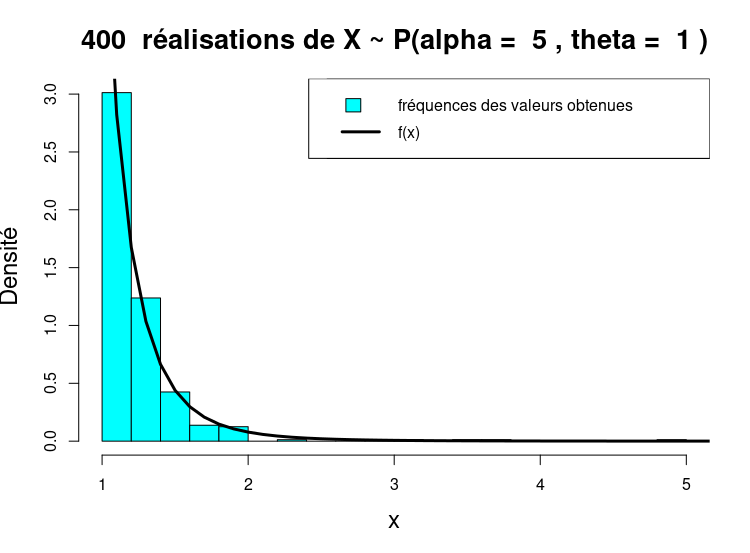
\includegraphics[width=11cm]{plot_hist_2_a5}
\caption{D'autres simulations d'une variable $X \sim \mathcal{P}(\alpha=5,\theta=1)$}
\end{center}
\end{figure}

\clearpage

\begin{figure}[!ht]
\begin{center}
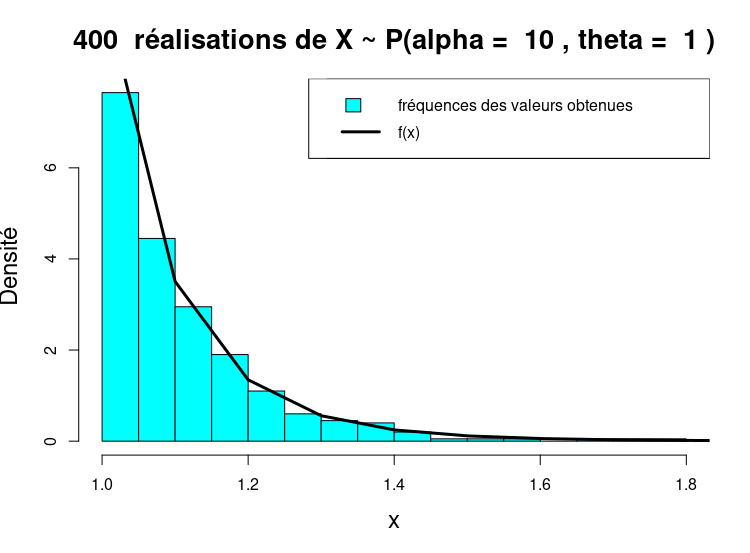
\includegraphics[width=11cm]{plot_hist_1_a10}
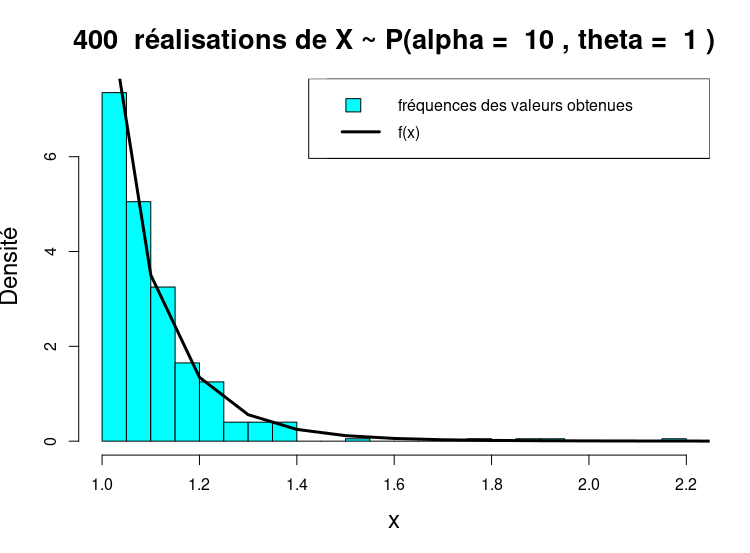
\includegraphics[width=11cm]{plot_hist_2_a10}
\caption{D'autres simulations d'une variable $X \sim \mathcal{P}(\alpha=10,\theta=1)$}
\end{center}
\end{figure}

\clearpage

\begin{figure}[!h]
\begin{center}
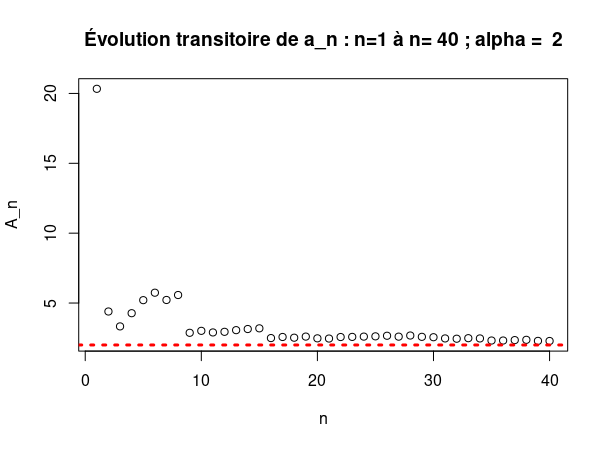
\includegraphics[width=6cm]{plot_graphique_transi_1}
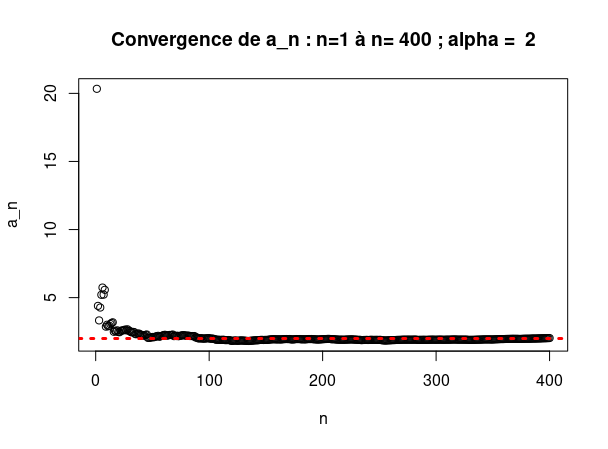
\includegraphics[width=6cm]{plot_graphique_conv_1}
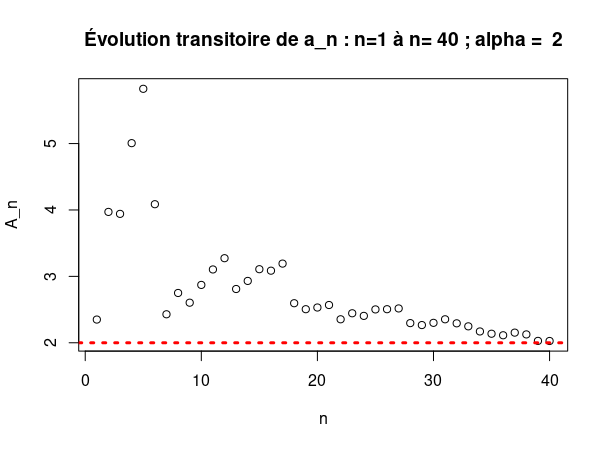
\includegraphics[width=6cm]{plot_graphique_transi_2}
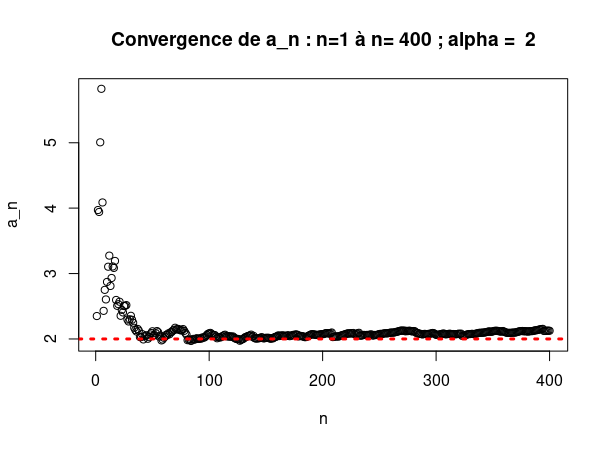
\includegraphics[width=6cm]{plot_graphique_conv_2}
\caption{Affichage des courbes d'évolution de $a_n$ lors d'exécutions différentes pour $\alpha=2$}
\end{center}
\end{figure}

\clearpage

\begin{figure}[!h]
\begin{center}
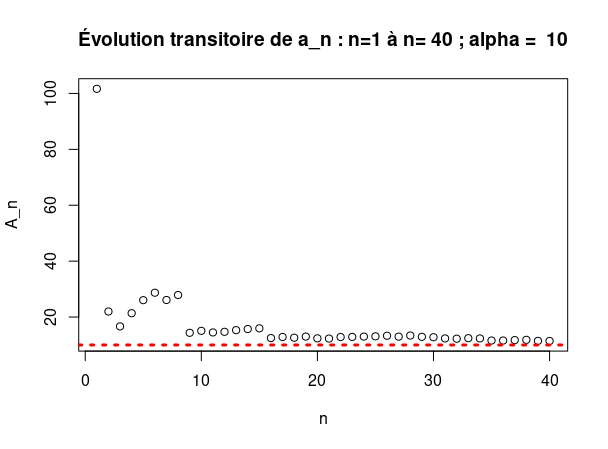
\includegraphics[width=6cm]{plot_graphique_transi_1_a10}
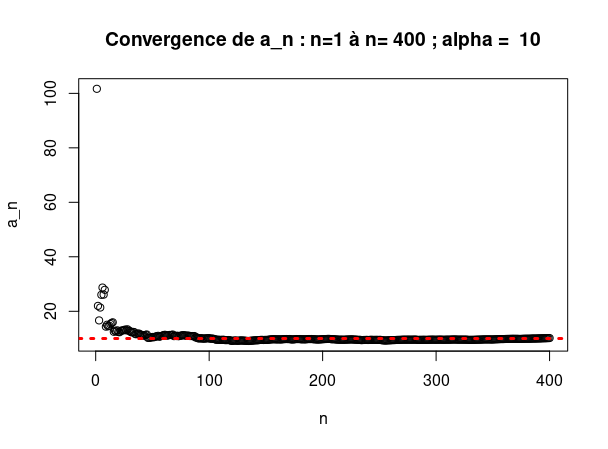
\includegraphics[width=6cm]{plot_graphique_conv_1_a10}
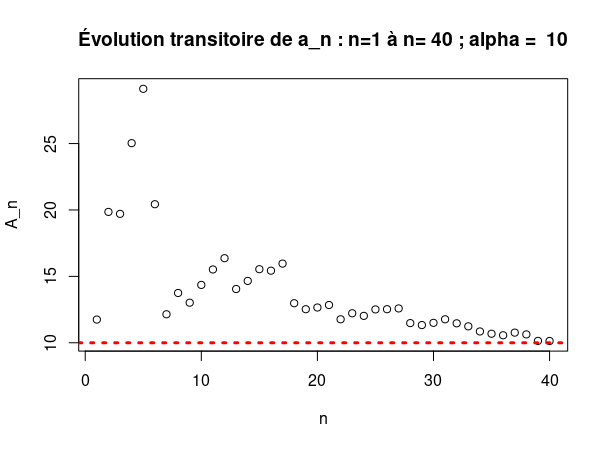
\includegraphics[width=6cm]{plot_graphique_transi_2_a10}
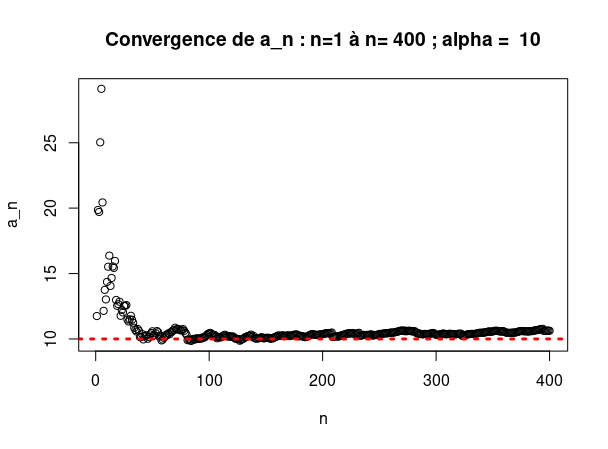
\includegraphics[width=6cm]{plot_graphique_conv_2_a10}
\caption{Affichage des courbes d'évolution de $a_n$ lors d'exécutions différentes pour $\alpha=10$}
\end{center}
\end{figure}

\clearpage

\begin{figure}[!h]
\begin{center}
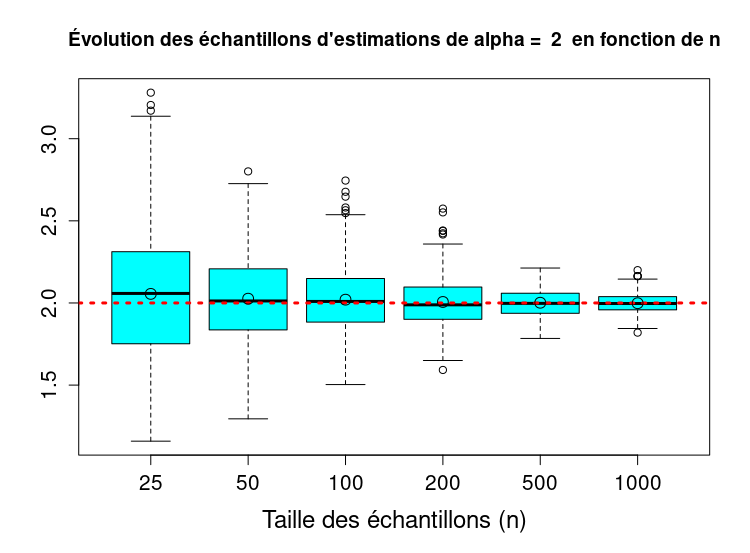
\includegraphics[width=11cm]{plot_box_1}
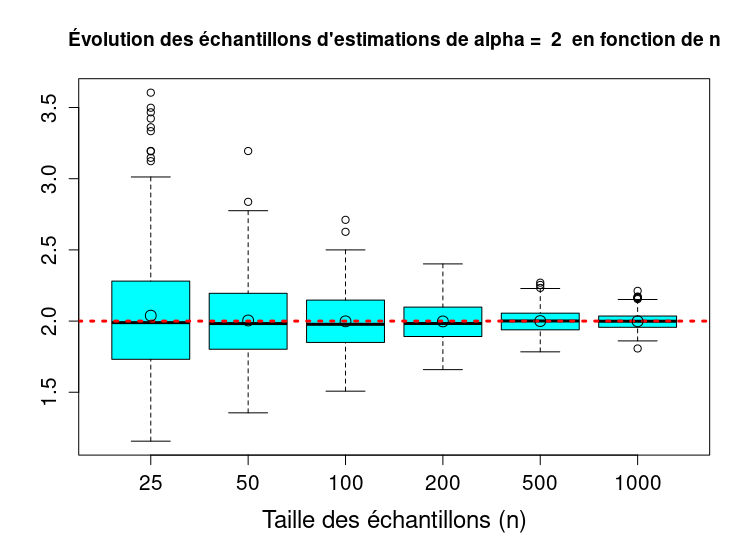
\includegraphics[width=11cm]{plot_box_2}
\caption{Représentation d'autres échantillons d'estimations de $\alpha=2$ par des boîtes à moustaches}
\end{center}
\end{figure}

\clearpage

\begin{figure}[!h]
\begin{center}
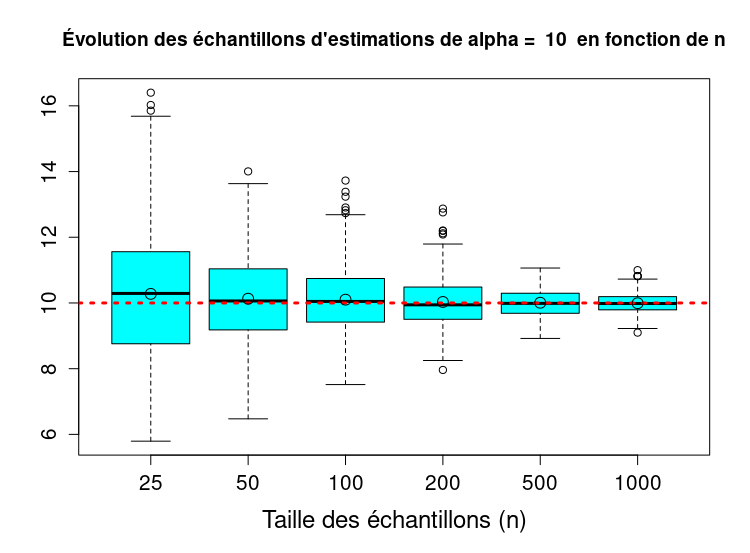
\includegraphics[width=11cm]{plot_box_1_a10}
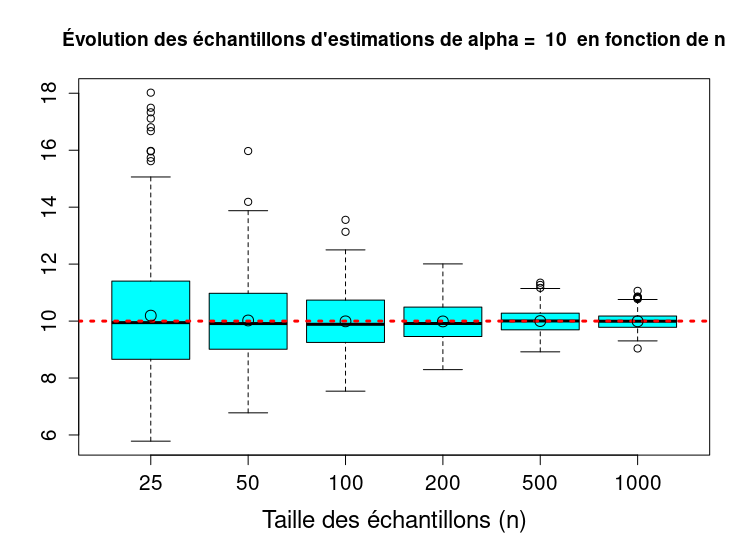
\includegraphics[width=11cm]{plot_box_2_a10}
\caption{Représentation d'autres échantillons d'estimations de $\alpha=10$ par des boîtes à moustaches}
\end{center}
\end{figure}

\subsection{Listing du programme R}

\begin{itemize}
\item[-] RNGkind(), set.seed(int) : initialisation de la graine de génération aléatoire de nombres
\item[-] runif($n$) : échantillon de $n$ simulations de la loi uniforme sur $[0,1]$
\item[-] paste(chaines) : concaténation de chaînes de caractères 
\item[-] hist() : construction d'un histogramme
\item[-] seq(deb,fin,pas) : génération d'un tableau de nombres de "deb" à "fin" espacés de "pas"
\item[-] lines($t$,$f(t)$) : tracé des valeurs $f(t)$ sur les points $t$ ($t$ est un tableau d'abscisses) 
\item[-] legend() : génération d'une légende sur le graphique obtenu
\item[-] matrix() : création d'une matrice
\item[-] plot($A$) : affichage des valeurs contenues dans la matrice $A$ sous la forme d'un graphique de points
\item[-] abline() : tracé d'une ligne sur le graphique
\item[-] boxplot() : affichage d'un histogramme
\item[-] points() : affichage de points sur un grahpique
\end{itemize}

\end{document}
